% !TeX TS-program = XeLaTex
% !TeX encoding = UTF-8
\documentclass[12pt]{beamer}
\usepackage{hyperref}
\usepackage[UTF8,noindent,fontset=]{ctex}
\usepackage{mathrsfs,tikz,xcolor,fontspec,graphicx,tcolorbox}
\usepackage{latexsym,amsmath,multicol,booktabs,calligra}
\usepackage{pstricks,listings,stackengine}
\usepackage{caption}
\usefonttheme[onlymath]{serif}
\usepackage[T1]{fontenc}
% \usepackage{concmath}
\usepackage{subfigure}
% \setCJKsansfont[ItalicFont=方正楷体_GBK.TTF]{方正苏新诗柳楷简体.TTF}
%\setCJKsansfont{方正宋刻本秀楷_GBK}
%\setCJKsansfont{Source Han Sans CN}
%\setCJKmainfont{Source Han Serif CN}
% \setCJKmainfont[BoldFont=方正小标宋_GBK.TTF]{方正新书宋_GBK.TTF}
%\usepackage[orientation=landscape,size=custom,width=16,height=9,scale=0.5,debug]{beamerposter}
\usepackage[en-GB]{datetime2} % Load the datetime2 package with English (UK) settings
%Modify the scale
\usetikzlibrary{arrows.meta,bending}
\usetheme{Madrid}
\usecolortheme{beaver}
%Page footer
\setbeamertemplate{footline}{
  \leavevmode%
  \hbox{%
    \begin{beamercolorbox}[wd=.333\paperwidth,ht=2.25ex,dp=1ex,center]{author in head/foot}
      \usebeamerfont{author in head/foot}\insertshortauthor
    \end{beamercolorbox}%
    \begin{beamercolorbox}[wd=.333\paperwidth,ht=2.25ex,dp=1ex,center]{title in head/foot}
      \usebeamerfont{title in head/foot}\insertshorttitle
    \end{beamercolorbox}%
    \begin{beamercolorbox}[wd=.333\paperwidth,ht=2.25ex,dp=1ex,right]{date in head/foot}
      \usebeamerfont{date in head/foot}\insertshortdate{}\hspace*{2em}
      \insertframenumber{} / \inserttotalframenumber\hspace*{2ex}
    \end{beamercolorbox}%
  }%
  \vskip0pt%
}
\setbeamercolor{author in head/foot}{fg=white, bg=yaublue}  %Footer author color
\setbeamercolor{title in head/foot}{fg=yaublue, bg=gray!180!black}  %Footer title color 
\setbeamercolor{date in head/foot}{fg=yaublue, bg=gray!170!black}  %Footer date color
\title{My Presentation} 
\author{Author's name}
% Set the date style to ISO format (YYYY-MM-DD)}
\date[\today]{\footnotesize\today}

\AtBeginSection[]
{
	\begin{frame}{Main content:}
		\transfade%Fade in and fade out effect
		\tableofcontents[sectionstyle=show/shaded] %I don't know exactly how to interpret these parameters, but the end result is to highlight the current chapter and fade the others
		\addtocounter{framenumber}{-1}  %Table of contents pages do not count page numbers
	\end{frame}
}
% \definecolor{yaured}{cmyk}{0,1,1,0.45}
\definecolor{yaublue}{RGB}{0,112,192}
\definecolor{yaured}{RGB}{0,122,192}
\definecolor{uired}  {HTML}{db3f3d}
\definecolor{uiblue} {HTML}{4ea0b7}
\definecolor{uigreen}{HTML}{789a5b}
\definecolor{uigray} {gray}{0.95}
\definecolor{uilink} {HTML}{00769E}%Define the color
\setbeamercolor{titlelike}{fg=yaublue}
\setbeamercolor{structure}{fg=yaublue}
\setbeamercolor{block body} {bg = uigray}
\setbeamercolor{block title}{fg = white,bg = yaublue!80}
\setbeamercolor{caption name}{fg=yaublue}
\setbeamercolor*{item projected}{fg=white, bg=yaublue!80!white}%Color settings
\begin{document}
\begin{frame}
% Add your logo in the bottom right corner
% \logo{\includegraphics[width=2cm]{YAUWZ9.png}}
%\usetheme{cambridgeUS}
\title[1234]{Yan'an University\\Yan'an University English beamer template}
%Multiple authors and affiliations
\author{Zhen Wang\inst{1} \and Yijie Zhu\inst{2}}
\institute[123]{\small {\inst{1}School of Mathematics and Computer Science\and
 \inst{2} Affiliation of the 2nd author}}




	
	    %\vspace{2cm}
		%\begin{center}
		%\resizebox{16em}{14pt}{\color{red!80} A brief introduction to Field-Feynman recursive model}\end{center}
		\begin{tikzpicture}[remember picture, overlay]
            \node[opacity=0.1] at ([shift={(0cm,-7.8cm)}]current page.north) {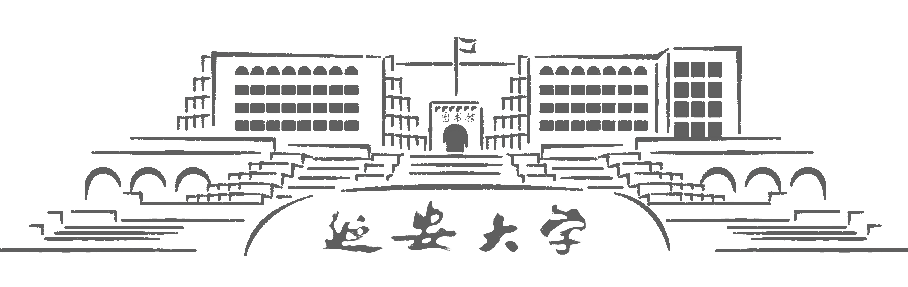
\includegraphics[width=10cm]{picture one.png}};
        \end{tikzpicture}
		\titlepage
	\end{frame}
	
	
	%Add a logo in the upper right corner
	\addtobeamertemplate{frametitle}{}{%
        \begin{tikzpicture}[remember picture,overlay]
        \node[anchor=north east,yshift=2pt] at (current page.north east) {
\includegraphics[height=0.8cm]{picture two.png}};
        \end{tikzpicture}}
	
	\section{Brief introduction}
	\begin{frame}{Brief introduction}
			\begin{tikzpicture}[remember picture, overlay]
            \node[opacity=0.05] at ([shift={(4cm,-6.8cm)}]current page.north) {
\includegraphics[width=3.5cm]{picturre three.png}};
        \end{tikzpicture}
	    The Madrid theme was used.
	\end{frame}
	
	\section{Insert formulas and blocks}
	\begin{frame}{Insert a formula}
	    Mean inequality
	    \[\frac{a+b}{2}\geqslant\sqrt{ab}.\]
	\end{frame}
	
	\begin{frame}{Insert a block}
	    \begin{block}{Newton's First Law}
			The object will remain in a uniform linear motion or at rest when it is not subjected to an external force.    
	    \end{block}
	\end{frame}
	
	\section{Insert a picture}
	\begin{frame}{Insert a picture}
	    \begin{figure}
	        \centering
	        
\includegraphics[width=0.5\textwidth]{picture four.png}
	        \caption{School Badge}
	        \label{fig1}
	    \end{figure}
	\end{frame}
	
	\beamertemplateshadingbackground{structure.fg!90}{structure.fg}
    \begin{frame}[plain]
    	\vfill
    	\centering
    	{
    		\centering \Huge \color{white}Thank you!
    	}
    	\vfill
    \end{frame}

\end{document}
